\chapter{Lissage Avancé, Ondelettes et Modèles Additifs}
\section{Smoothing Splines (Splines de Lissage)}

\subsection{Problématique et Motivation}
L'approche des splines de régression nécessite de choisir le nombre et la position des nœuds. Une alternative consiste à chercher une fonction $f$ qui ajuste bien les données tout en étant "lisse". Si nous minimisons simplement le RSS sans contraintes, nous obtenons une fonction qui interpole tous les points de données, conduisant à un sur-apprentissage massif.

\begin{figure}[h]
    \centering
    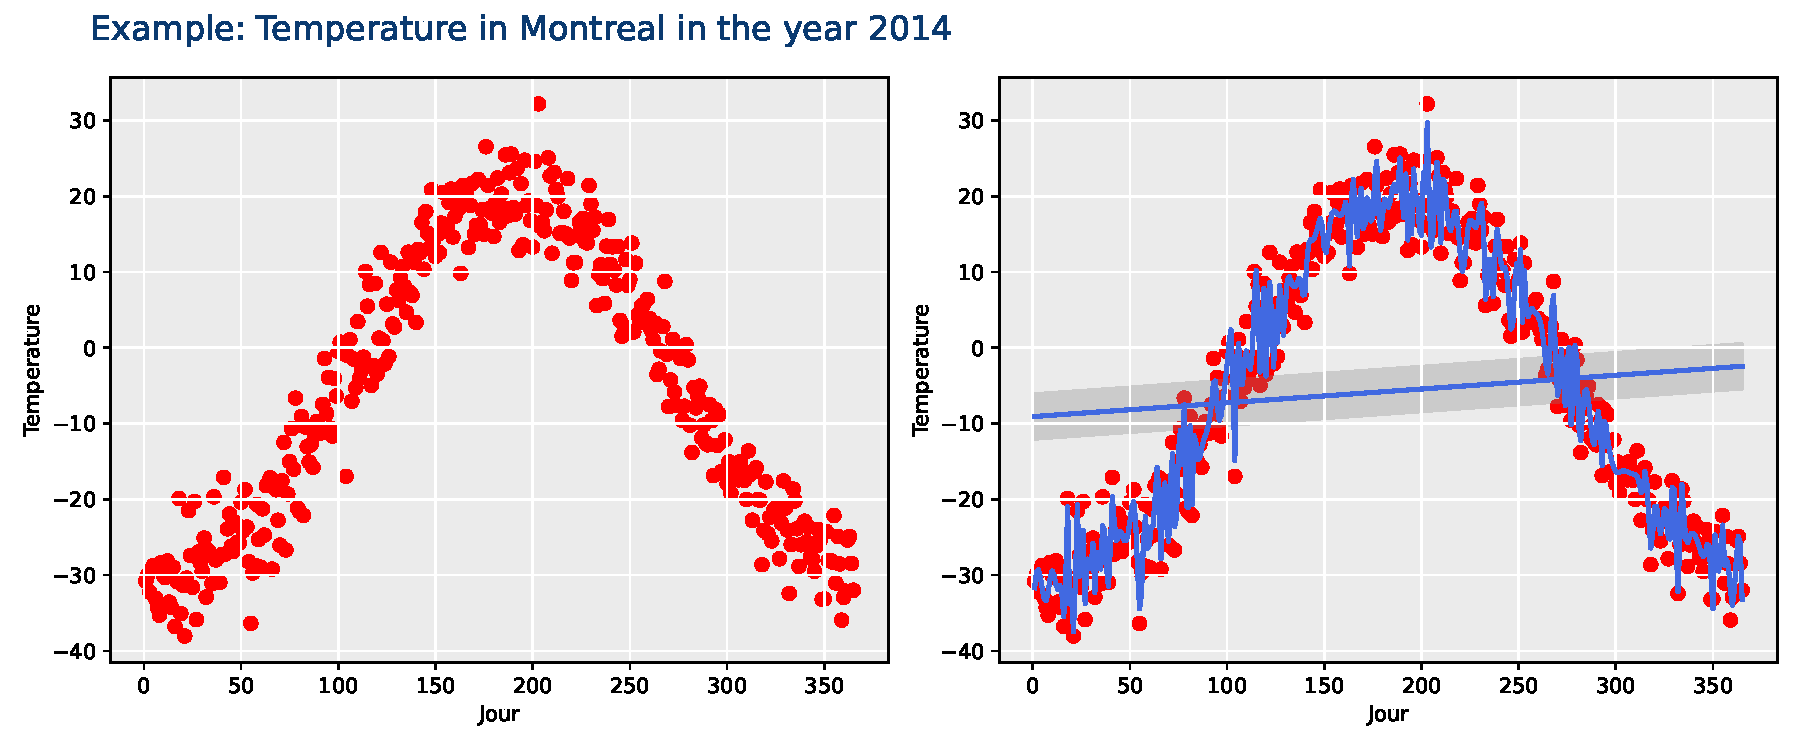
\includegraphics[width=\textwidth]{images/montreal_temp.pdf}
    \caption{Exemple de lissage de la température à Montréal en fonction du temps. Une spline de lissage permet de capturer la tendance non-linéaire mieux qu'un modèle linéaire ou polynomial simple.}
    \label{fig:montreal_temp}
\end{figure}

\subsection{Critère de Minimisation}
La spline de lissage est la fonction $f$ qui minimise le critère suivant:
\begin{equation}
    \sum_{i=1}^{n} (y_i - f(x_i))^2 + \lambda \int f''(t)^2 dt
\end{equation}
\begin{itemize}
    \item \textbf{Terme de fidélité aux données} : $\sum (y_i - f(x_i))^2$ (RSS).
    \item \textbf{Pénalité de rugosité} : $\lambda \int f''(t)^2 dt$ pénalise la variabilité de $f$ (sa courbure).
    \item \textbf{Paramètre de réglage $\lambda$} : Contrôle le compromis. Si $\lambda=0$, $f$ interpole les données ; si $\lambda \to \infty$, $f$ devient une droite (moindres carrés linéaires).
\end{itemize}

\begin{figure}[h]
    \centering
    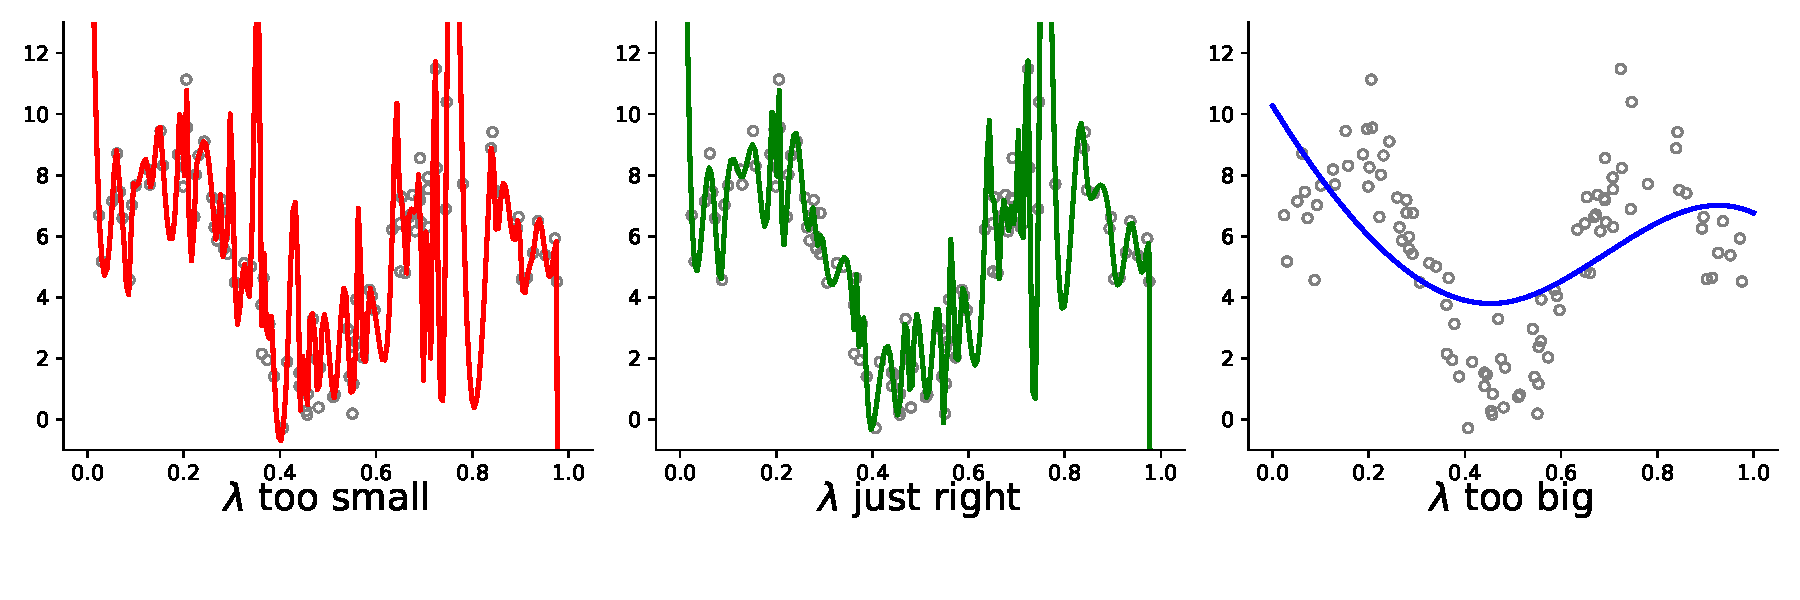
\includegraphics[width=\textwidth]{images/smoothing_spline_lambda.pdf}
    \caption{L'effet du paramètre de réglage $\lambda$ sur une spline de lissage. De gauche à droite: $\lambda$ trop petit (sur-apprentissage), $\lambda$ optimal, $\lambda$ trop grand (sous-apprentissage).}
    \label{fig:smoothing_spline_lambda}
\end{figure}
\subsection{Propriétés et Solution}
Il est remarquable que pour tout $\lambda > 0$, la solution unique est une \textbf{spline cubique naturelle} possédant des nœuds en chaque point d'observation $x_1, \dots, x_n$. Cependant, il s'agit d'une version "réduite" (shrunken) par rapport à une spline de régression classique sur ces mêmes nœuds.

La solution s'écrit sous forme matricielle:
\begin{equation}
    \hat{\beta} = (N^T N + \lambda \Omega_N)^{-1} N^T Y
\end{equation}
où $N$ est la matrice de base des splines et $\Omega_N$ la matrice de pénalité.

\subsection{Degrés de liberté effectifs}
Contrairement aux splines de régression, le nombre de nœuds n'est plus le paramètre de complexité. On utilise les \textbf{degrés de liberté effectifs} $df_\lambda$, définis par la trace de la matrice de lissage $S_\lambda$:
\begin{equation}
    df_\lambda = \text{tr}(S_\lambda)
\end{equation}
Le choix de $\lambda$ (ou de $df_\lambda$) est crucial et s'effectue généralement par validation croisée (LOOCV). Plus $\lambda$ est grand, plus la pénalité est forte, ce qui réduit les degrés de liberté effectifs $df_\lambda$ et force la courbe à s'aplatir vers une droite linéaire ($df \to 2$). À l'inverse, un $\lambda \to 0$ donne $df_\lambda \to n$ (interpolation parfaite).

\section{Régression par Ondelettes (Wavelet Regression)}

\subsection{Représentations Temps-Fréquence}
La motivation des ondelettes vient de l'incapacité de la transformée de Fourier à localiser les changements de régime dans le temps. 
\begin{itemize}
    \item \textbf{Fourier} : Excellente résolution fréquentielle, aucune localisation temporelle.
    \item \textbf{Fenêtrage (Gabor)} : Utilise une fenêtre fixe, limitée par le principe d'incertitude de Heisenberg.
    \item \textbf{Ondelettes} : Utilise des fenêtres de tailles variables (dilatations), permettant une analyse multi-échelle.
\end{itemize}

\begin{figure}[h]
    \centering
    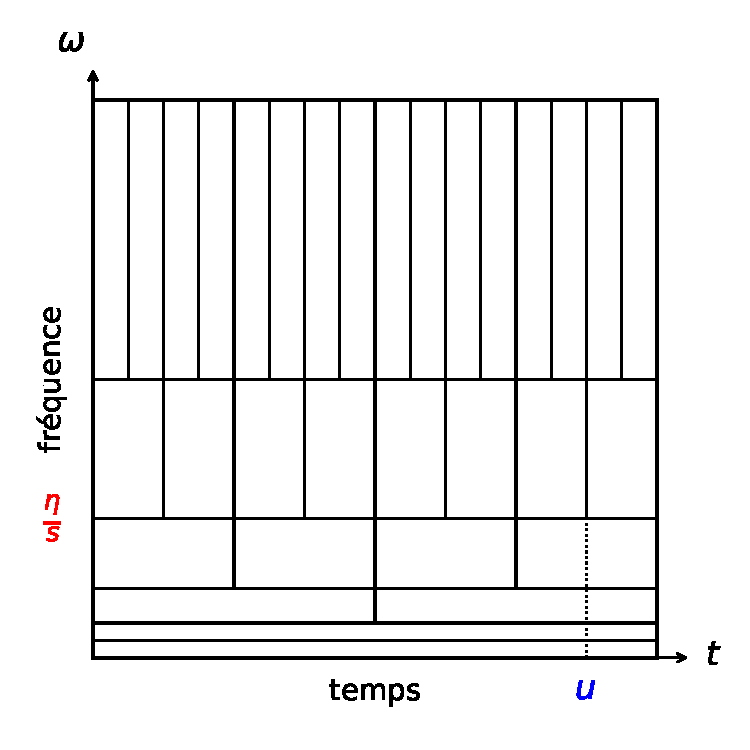
\includegraphics[width=0.6\textwidth]{images/wavelet_tiling.pdf}
    \caption{Pavage temps-fréquence d'une analyse par ondelettes. Les hautes fréquences ont une bonne résolution temporelle, tandis que les basses fréquences ont une bonne résolution fréquentielle.}
    \label{fig:wavelet_tiling}
\end{figure}

\begin{figure}[h]
    \centering
    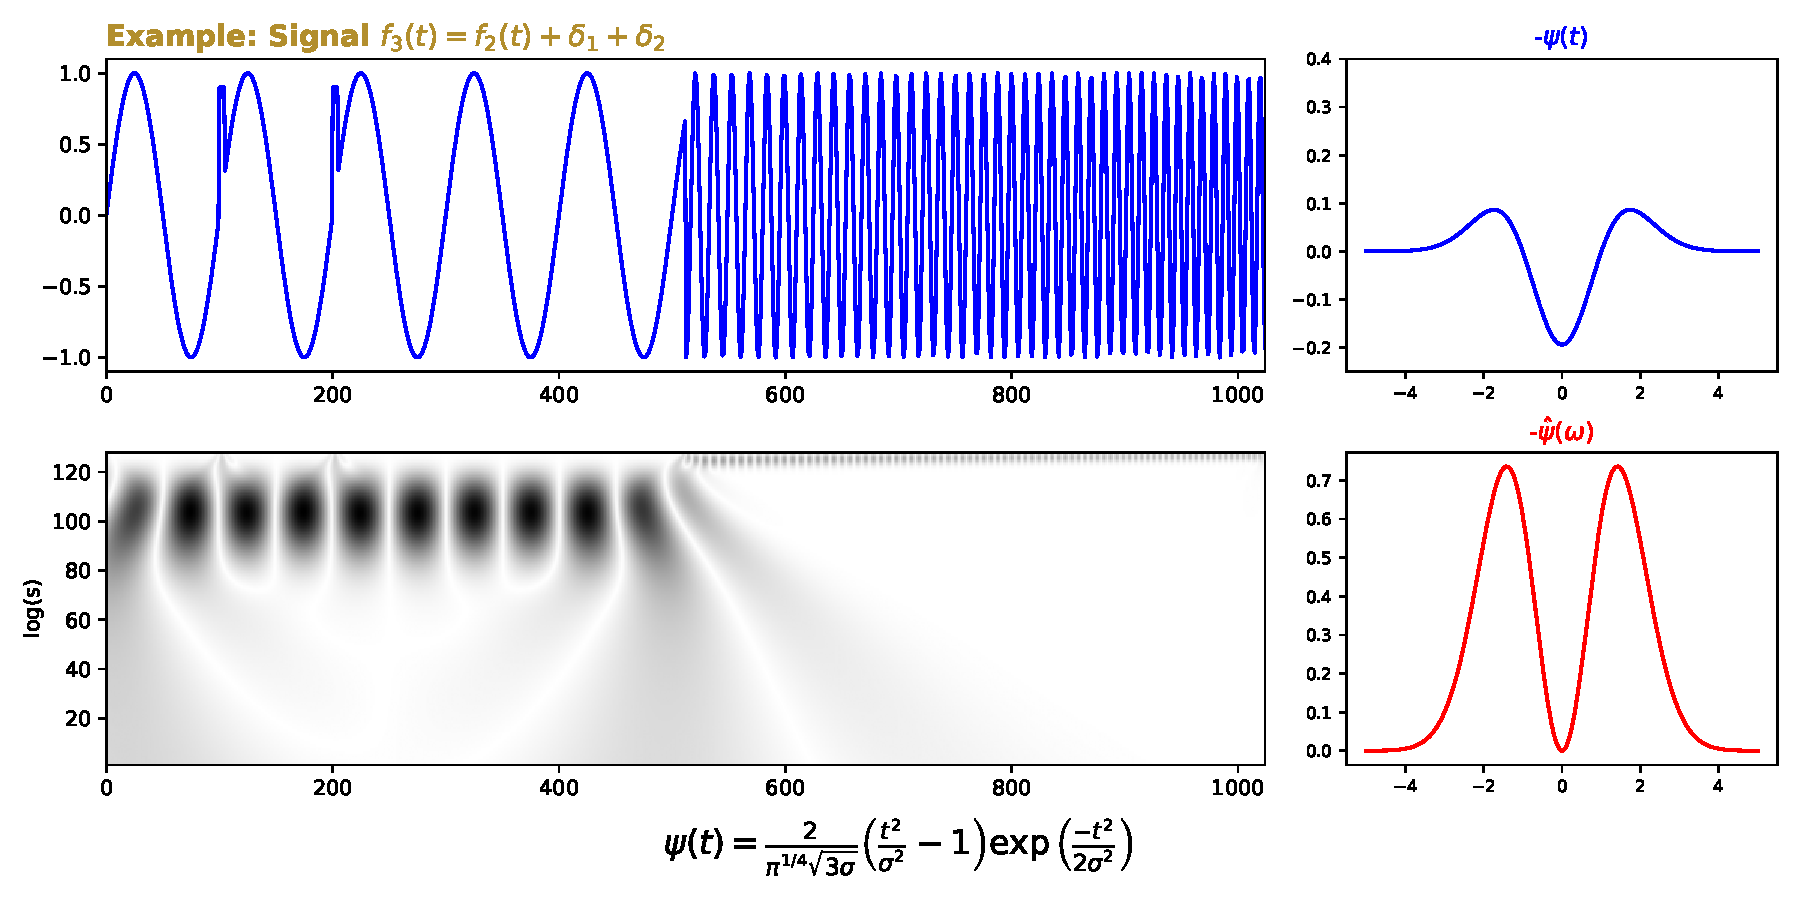
\includegraphics[width=\textwidth]{images/wavelet_signal_cwt.pdf}
    \caption{En haut, un signal non-stationnaire composé d'une onde sinusoïdale de basse fréquence, de deux sauts brusques, et d'un chirp. En bas, le scalogramme (CWT) illustrant la localisation temps-fréquence. À droite, les ondellettes (ex: Hat/Ricker).}
    \label{fig:wavelet_signal_cwt}
\end{figure}
\subsection{Définition d'une Ondelette}
Une ondelette $\psi$ est une fonction de moyenne nulle, centrée en 0. On génère une famille de fonctions par translation ($u$) et dilatation ($s$):
\begin{equation}
    \psi_{u,s}(t) = \frac{1}{\sqrt{s}} \psi\left(\frac{t-u}{s}\right)
\end{equation}

\subsection{Décomposition et Sparsité}
L'idée est de décomposer une fonction sur une base orthonormée d'ondelettes. L'exemple le plus simple est la base de \textbf{Haar}. 
Les ondelettes sont particulièrement efficaces car elles induisent de la \textbf{sparsité} : un petit nombre de coefficients suffit à représenter l'essentiel de l'information d'un signal ou d'une image (principe utilisé dans le format JPEG2000).

\begin{figure}[h]
    \centering
    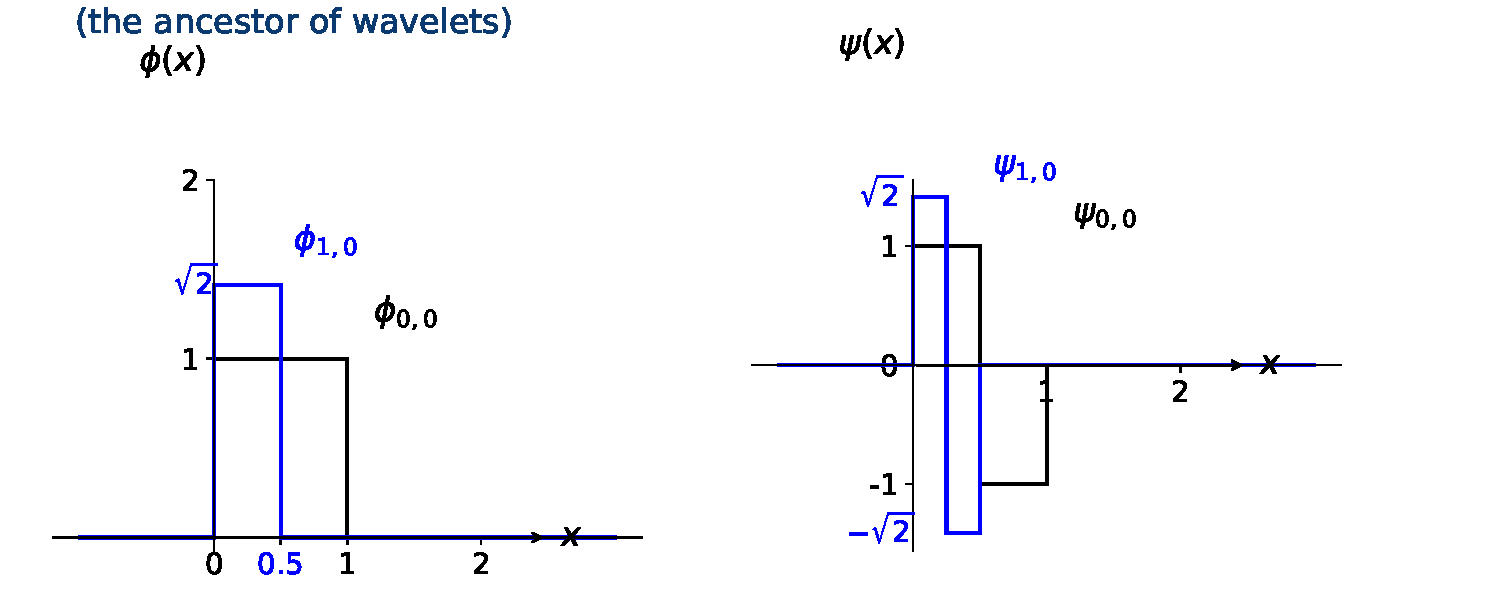
\includegraphics[width=\textwidth]{images/haar_basis_original.pdf}
    \caption{Fonction d'échelle $\phi(x)$ et ondelette de Haar $\psi(x)$, avec leurs premières versions translatées/dilatées.}
    \label{fig:haar_basis_original}
\end{figure}

\begin{figure}[h]
    \centering
    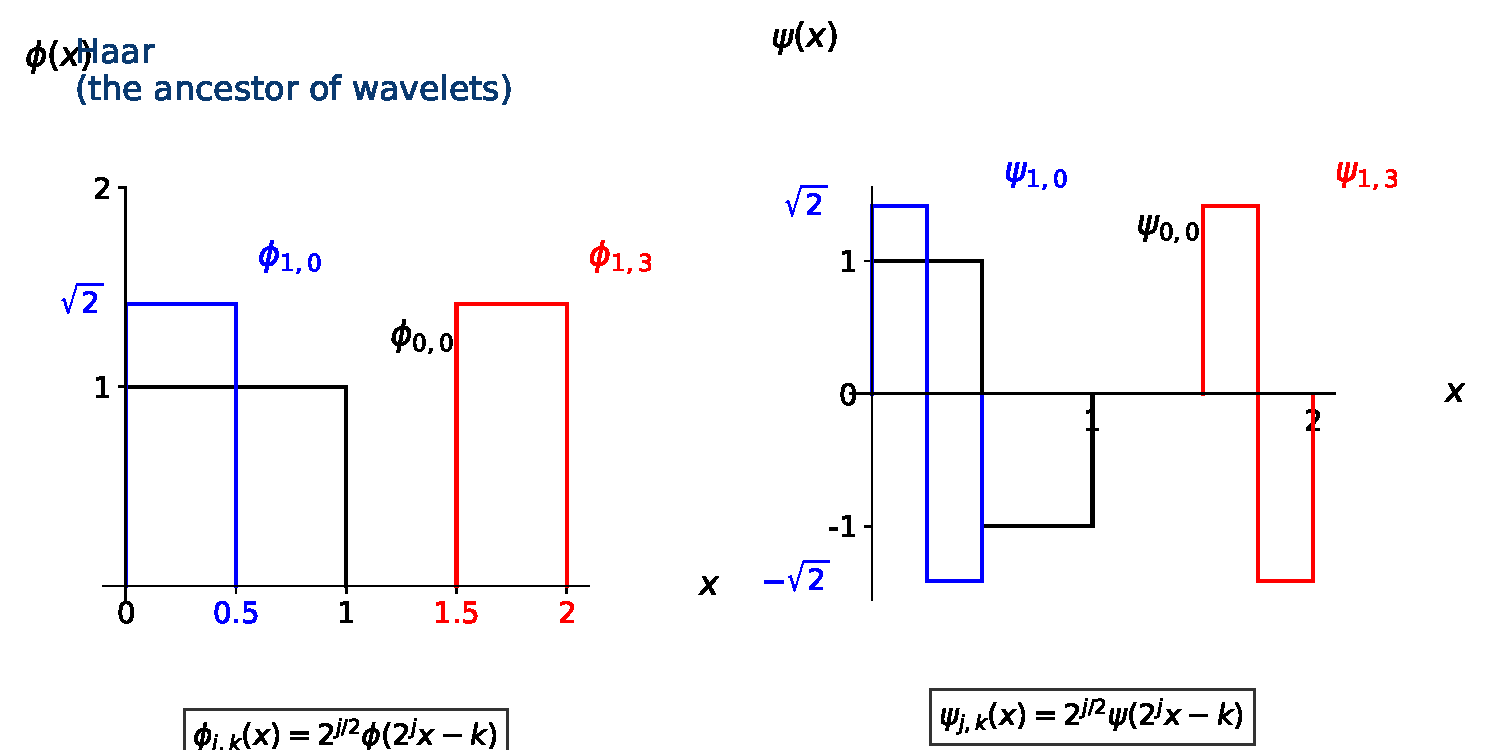
\includegraphics[width=\textwidth]{images/haar_basis_scaled.pdf}
    \caption{Exemples de l'échelonnement et la translation pour la base de Haar.}
    \label{fig:haar_basis_scaled}
\end{figure}

\begin{figure}[h]
    \centering
    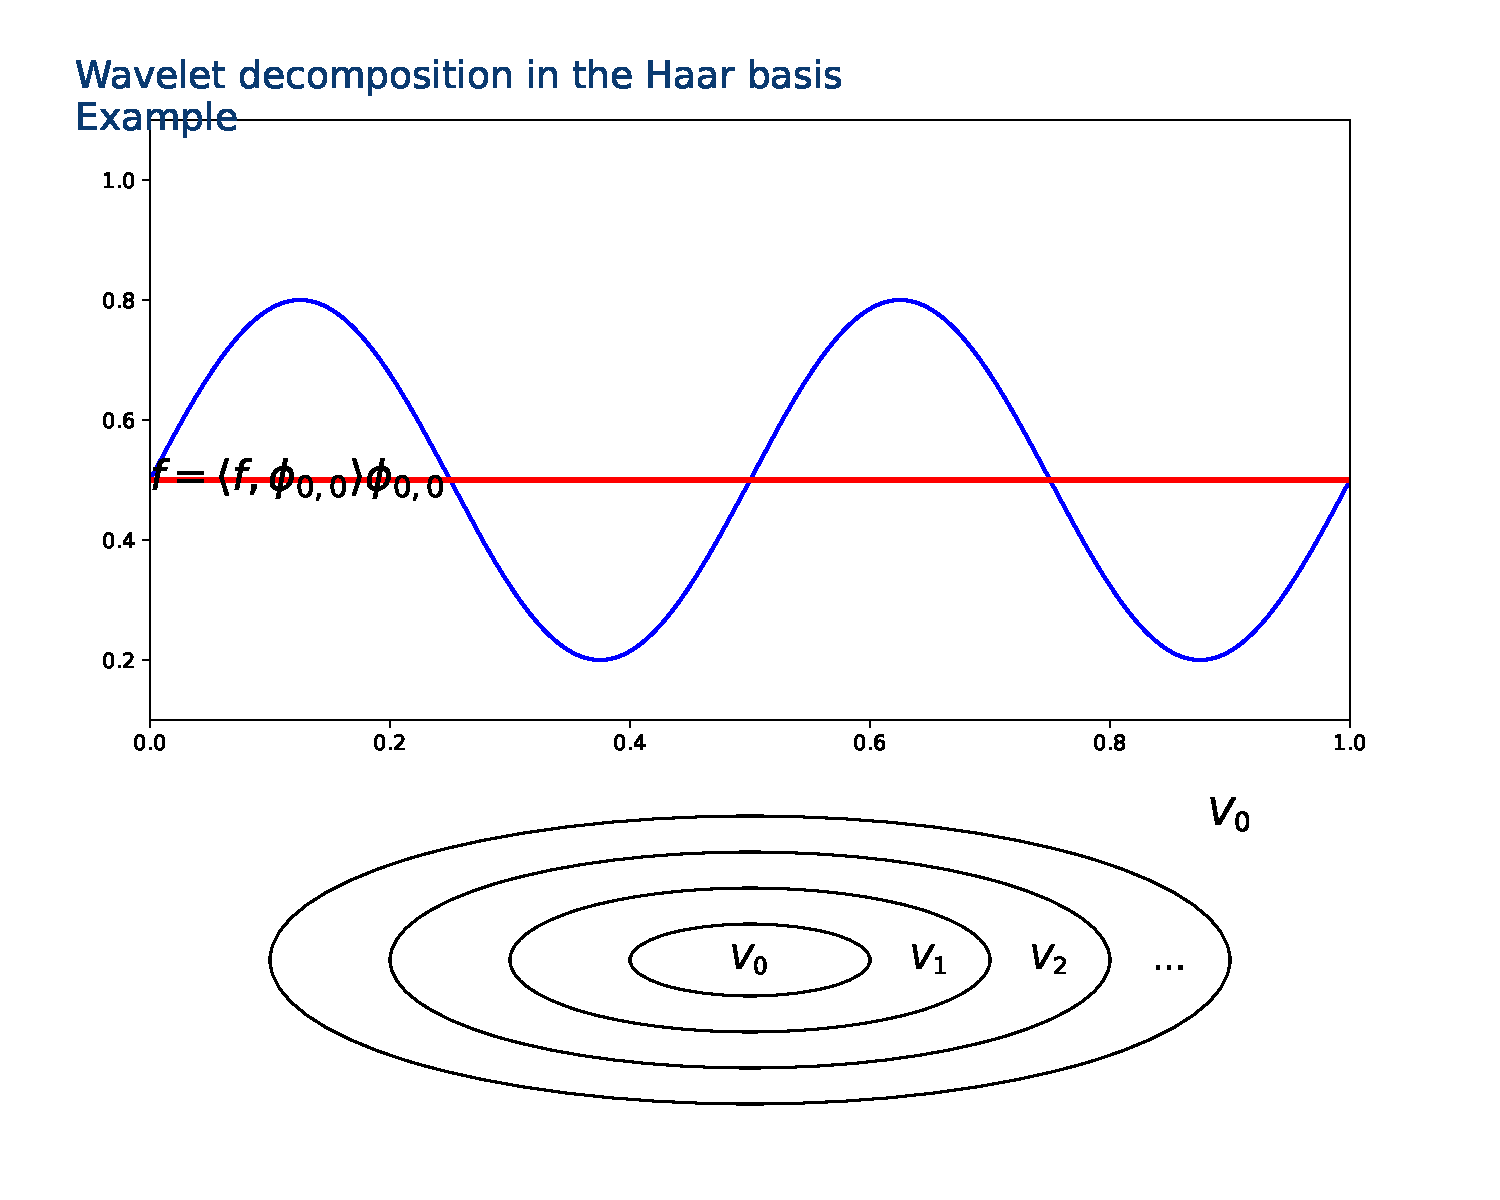
\includegraphics[width=0.8\textwidth]{images/haar_decomposition_V0.pdf}
    \caption{Décomposition en ondelettes : Projection sur l'espace d'approximation $V_0$.}
    \label{fig:haar_decomp_v0}
\end{figure}

\begin{figure}[h]
    \centering
    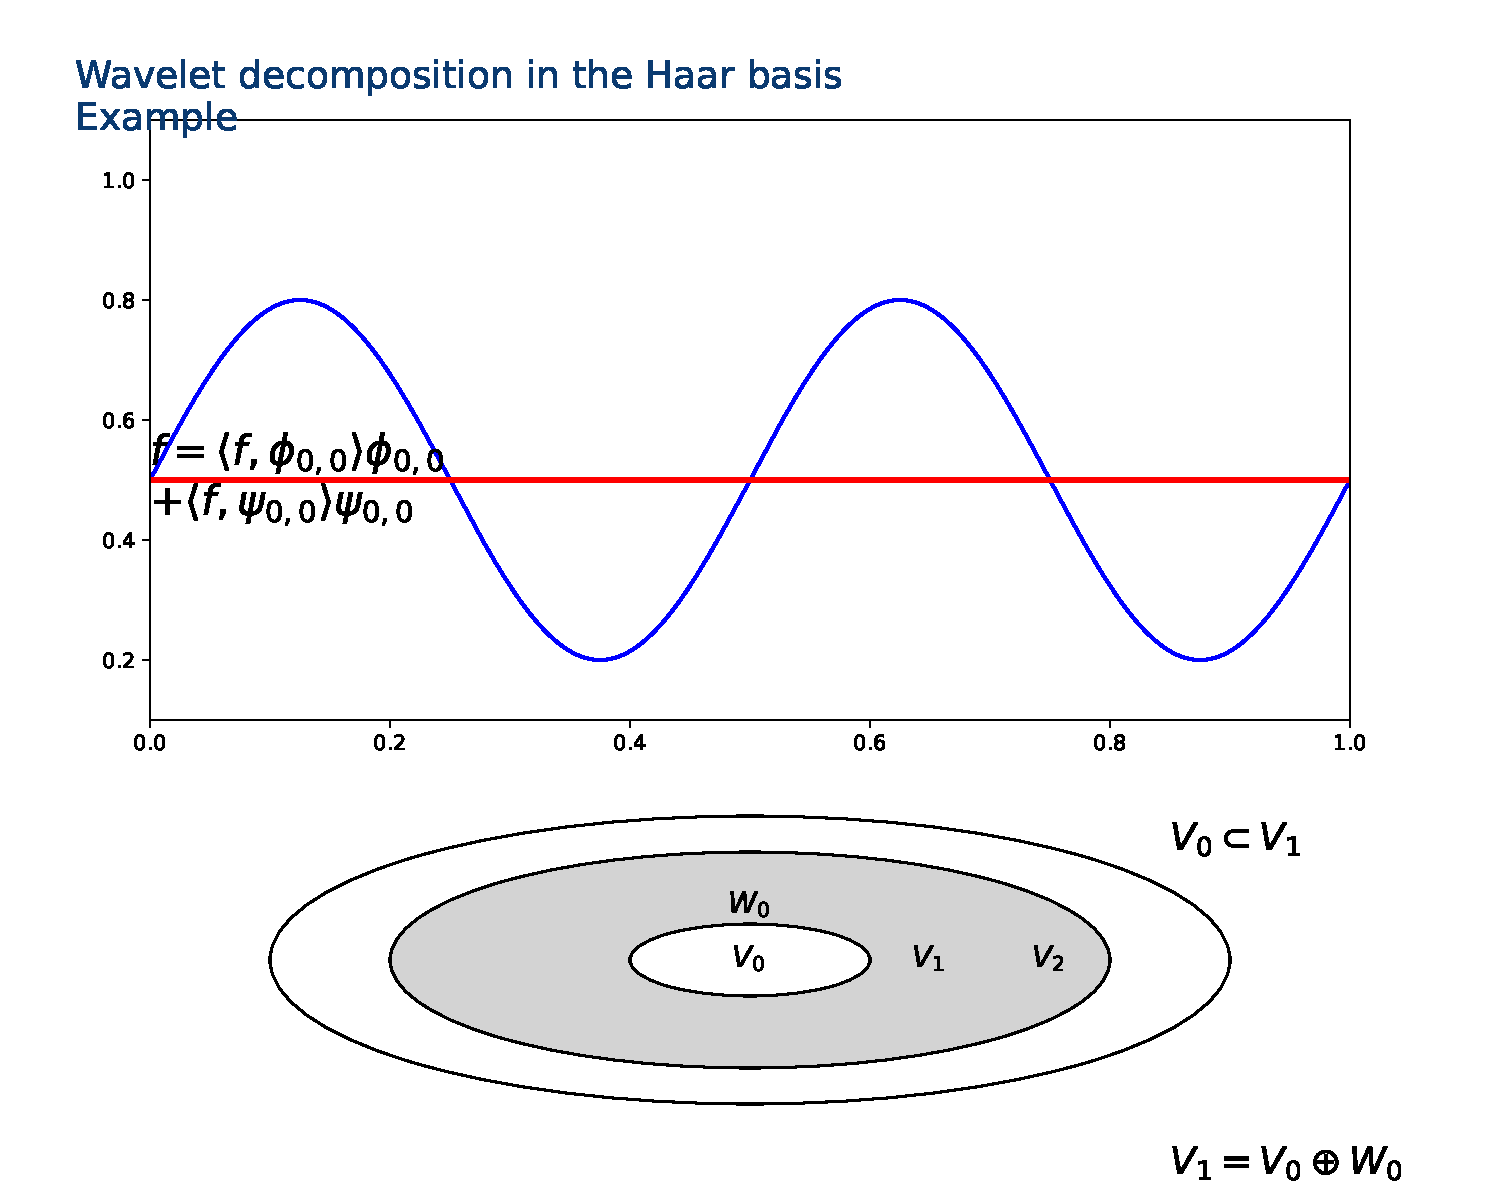
\includegraphics[width=0.8\textwidth]{images/haar_decomposition_V1_W0.pdf}
    \caption{Décomposition en ondelettes : Projection sur $V_1 = V_0 \oplus W_0$.}
    \label{fig:haar_decomp_v1_w0}
\end{figure}

\begin{figure}[h]
    \centering
    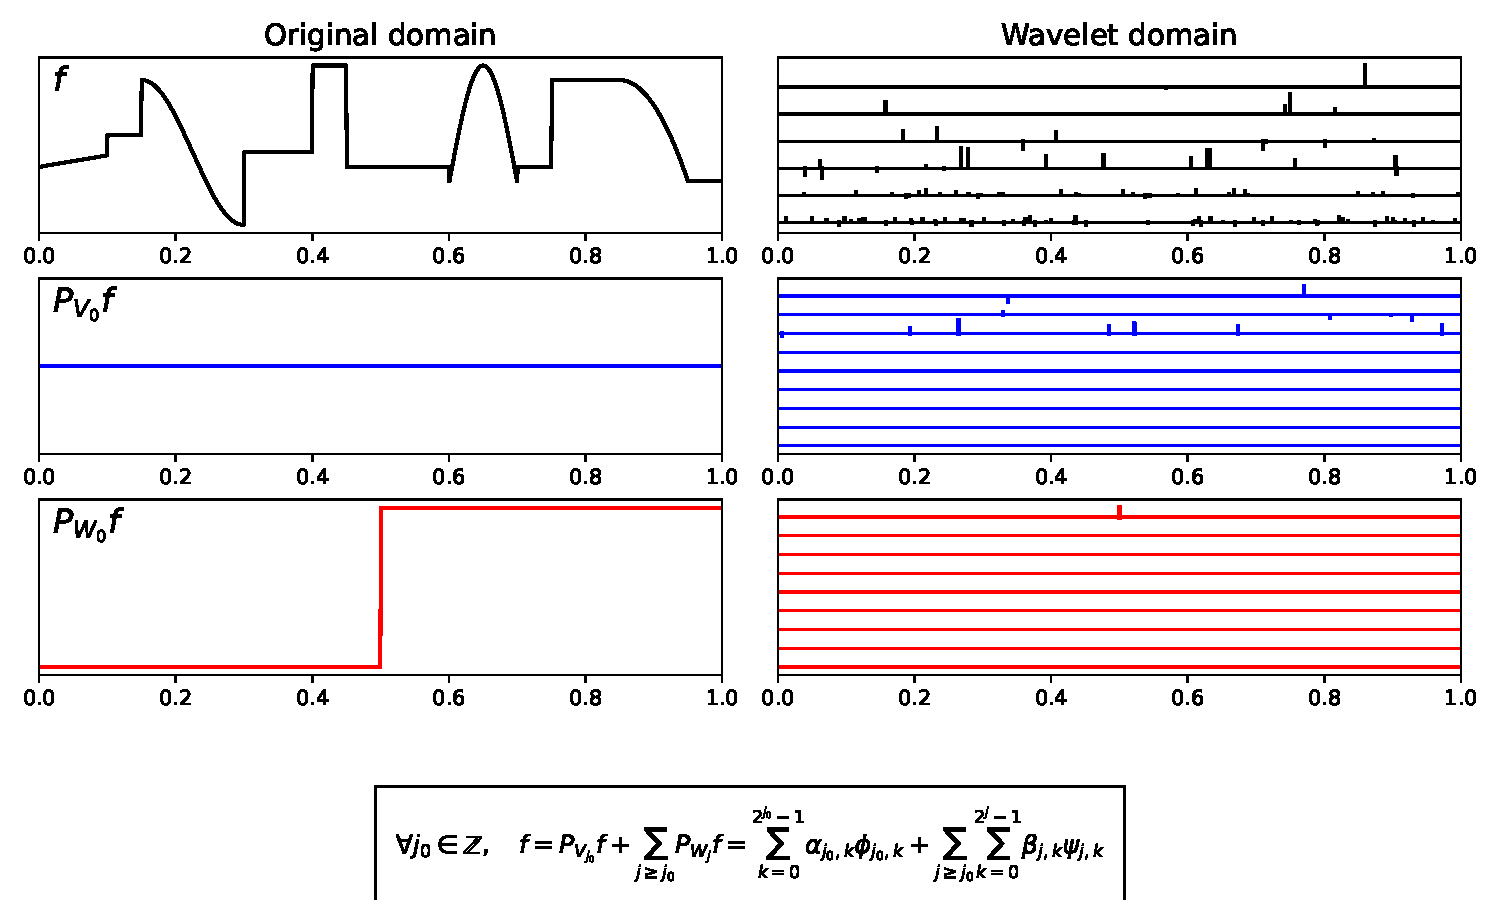
\includegraphics[width=\textwidth]{images/haar_domain_projections.pdf}
    \caption{Projection d'un signal (à gauche) et son équivalent dans le domaine des ondelettes (à droite), avec approximations et espaces de détails.}
    \label{fig:haar_domain_projections}
\end{figure}

\subsection{Débruitage par Seuillage (Thresholding)}
Dans un contexte de régression $Y_i = f(x_i) + \epsilon_i$, on estime $f$ en trois étapes:
\begin{enumerate}
    \item Calculer les coefficients d'ondelettes $\hat{\theta} = WY$ via une transformée rapide (DWT).
    \item Appliquer un \textbf{seuillage} sur les coefficients pour éliminer le bruit:
    \begin{itemize}
        \item \textbf{Seuillage dur} (Hard) : On annule les coefficients inférieurs à un seuil $\lambda$.
        \item \textbf{Seuillage doux} (Soft) : On réduit l'amplitude des coefficients conservés.
    \end{itemize}
    \item Appliquer la transformée inverse pour reconstruire le signal estimé $\hat{f}$.
\end{enumerate}
\textbf{($\bigstar$ EXAMEN)} C'est précisément cette étape de seuillage qui confère aux ondelettes leur pouvoir de \textbf{sparsité} (parcimonie). En forçant la majorité des petits coefficients de détail (souvent assimilables au bruit) à zéro pur, on obtient une représentation extrêmement compacte et lisse du signal original, tout en préservant intactes les caractéristiques locales majeures (comme les sauts ou les discontinuités fortes).

\section{Modèles Additifs Généralisés (GAM)}

\subsection{Définition}
Les GAM étendent la régression linéaire multiple en remplaçant chaque composante linéaire $\beta_j x_{ij}$ par une fonction non-linéaire lisse $f_j(x_{ij})$:
\begin{equation}
    y_i = \beta_0 + \sum_{j=1}^{p} f_j(x_{ij}) + \epsilon_i
\end{equation}
Le modèle reste \textbf{additif} car nous calculons une contribution séparée pour chaque variable avant de les sommer.

\subsection{Avantages et Limites}
\begin{itemize}
    \item \textbf{Avantages} : Modélisation automatique des relations non-linéaires, meilleure précision prédictive, et maintien de l'interprétabilité (on peut visualiser l'effet de chaque variable individuellement).
    \item \textbf{Limites} : L'additivité empêche de capturer les interactions complexes entre variables, à moins de les ajouter manuellement.
\end{itemize}

\subsection{\textbf{($\bigstar$ EXAMEN)} GAM pour la Classification (Régression Logistique)}
Contrairement à une idée répandue, les Modèles Additifs Généralisés ne se limitent absolument pas à la régression continue. Ils étendent directement la régression logistique à des relations non-linéaires lisses. Pour une variable cible qualitative, on modélise la probabilité $p(X)$ d'appartenir à une classe via la fonction de lien logit classique :
\begin{equation}
    \log\left(\frac{p(X)}{1-p(X)}\right) = \beta_0 + f_1(X_1) + \dots + f_p(X_p)
\end{equation}
Cela permet de bénéficier d'avantages non-linéaires en classification discrète tout en préservant l'interprétabilité marginale de la régression logistique "vanilla".

\subsection{Mise en œuvre en R}
On utilise principalement les packages \texttt{gam} ou \texttt{mgcv}:
\begin{itemize}
    \item \textbf{Avec splines naturelles} : \texttt{lm(y \textasciitilde ns(x1, df) + ns(x2, df), data)}.
    \item \textbf{Avec splines de lissage} : \texttt{gam(y \textasciitilde s(x1, df) + s(x2, df), data)}.
\end{itemize}
L'ajustement peut se faire par moindres carrés si les bases sont fixées, ou par l'algorithme de \textbf{backfitting} pour les splines de lissage.
